{\Large Bits bem escovados.}

\begin{enumerate}
	\item Conceito de informação: exemplo da fogueira (acesa/apagada.
	\item Unidades de medida de informação.
	\item Combinacões de possíveis mensagens com:
	\begin{enumerate}
		\item 1 bit (ou 1 luzinha!).
		\item 2 bits (2 luzinhas).
		\item 4 bits (4 luzinhas).
		\item 1 Byte (8 luzinhas).
		\item KiloB
		\item MegaB
		\item GigaB
		\item TeraB
		\item Utilizar múltiplos de 1000, nesta idade, ja que a matematica mais correta, com múltiplos de 1024, e complexa demais, nesta idade.
	\end{enumerate}
	\item Código ASCII.
\end{enumerate}

\begin{center}
	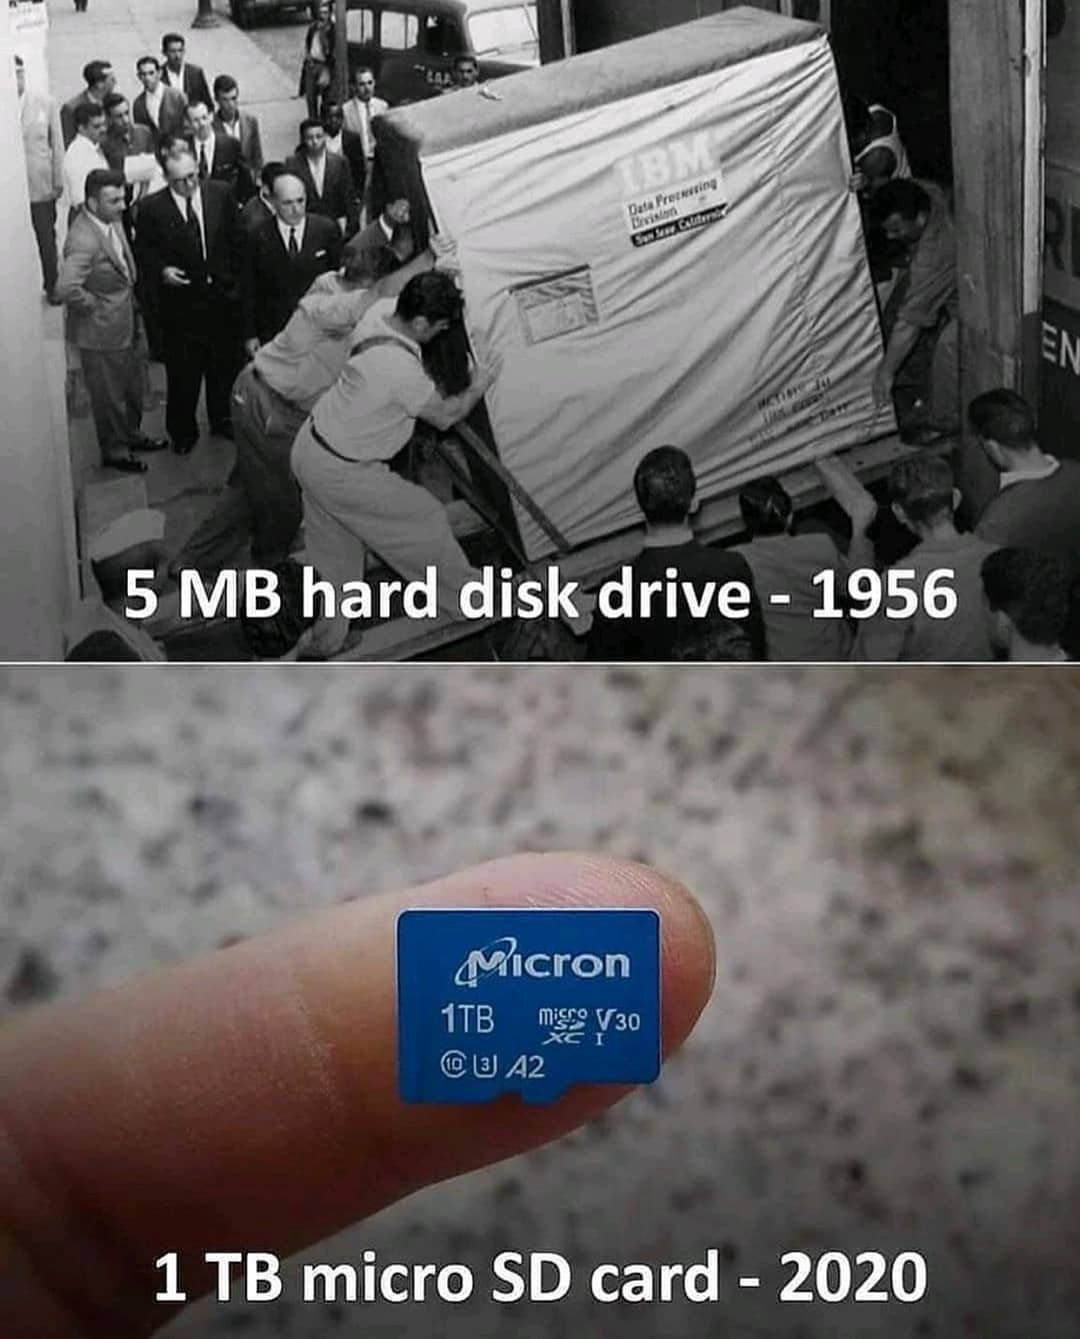
\includegraphics[width=.7\linewidth]{./IMG/hd-1956.jpg}
\end{center}

%\begin{center}
%	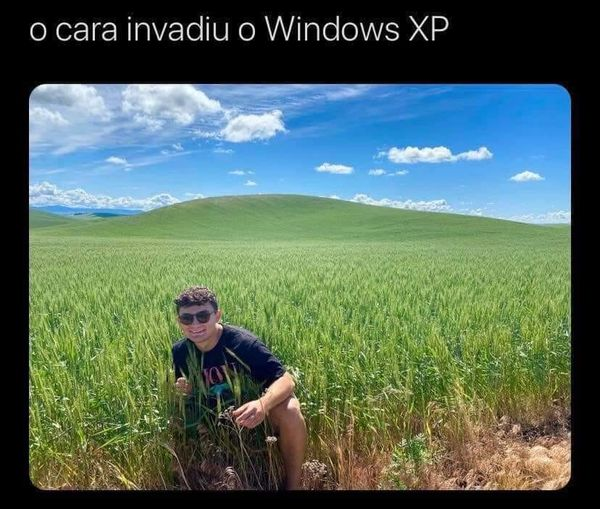
\includegraphics[width=\linewidth]{./I MG/xp.jpg}
%\end{center}

\vfill\null
\columnbreak
